\documentclass[multi={tikzpicture},border=8pt]{standalone}
\usepackage{tnviz}

\begin{document}

% 1. Orb: the same renderer is neutral gray by default and becomes coloured
% from one base-colour value.
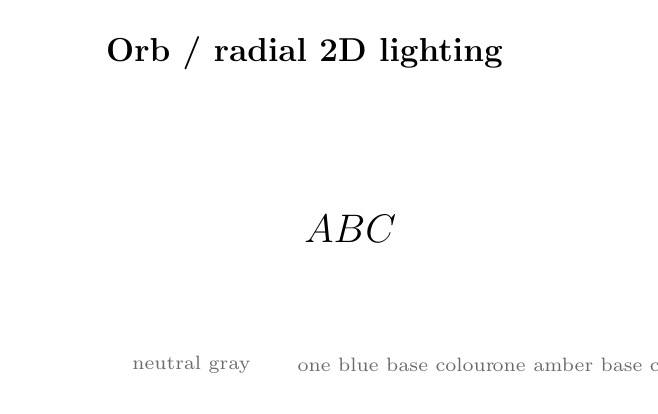
\begin{tikzpicture}[font=\sffamily]
  \node[font=\bfseries\large] at (0,2.4) {Orb / radial 2D lighting};
  \tnvShape[shape=orb,color=black!48,width=22mm,font=\Large]{orb-gray}{(-2.6,0)}{$A$}
  \tnvShape[shape=orb,color=blue!62!black,width=22mm,font=\Large]{orb-blue}{(0,0)}{$B$}
  \tnvShape[shape=orb,color=orange!78!black,width=22mm,font=\Large]{orb-amber}{(2.6,0)}{$C$}
  \node[font=\scriptsize,text=black!58] at (-2.6,-1.55) {neutral gray};
  \node[font=\scriptsize,text=black!58] at (0,-1.55) {one blue base colour};
  \node[font=\scriptsize,text=black!58] at (2.6,-1.55) {one amber base colour};
\end{tikzpicture}

% 2. Rectangle: radius zero is the sharp-corner form of the same glyph.
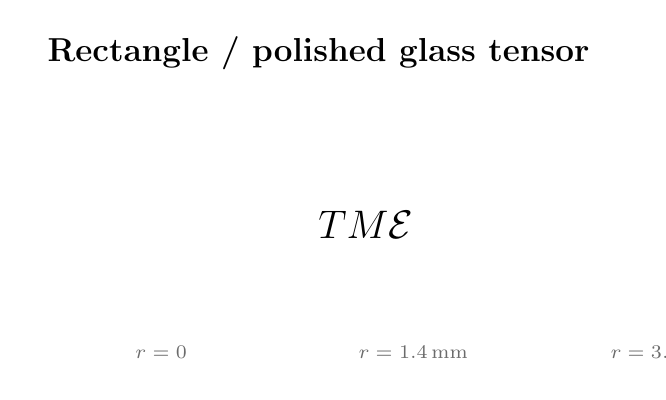
\begin{tikzpicture}[font=\sffamily]
  \node[font=\bfseries\large] at (0,2.35) {Rectangle / polished glass tensor};
  \tnvShape[shape=rounded rectangle,color=black!48,width=25mm,height=13mm,corner radius=0mm,font=\Large]{rect-sharp}{(-3.2,0)}{$T$}
  \tnvShape[shape=rounded rectangle,color=blue!64!black,width=25mm,height=13mm,corner radius=1.4mm,font=\Large,text color=white!92!black]{rect-soft}{(0,0)}{$M$}
  \tnvShape[shape=rounded rectangle,color=violet!64!black,width=25mm,height=13mm,corner radius=3.2mm,font=\Large,text color=white!92!black]{rect-round}{(3.2,0)}{$\mathcal{E}$}
  \node[font=\scriptsize,text=black!58] at (-3.2,-1.45) {$r=0$};
  \node[font=\scriptsize,text=black!58] at (0,-1.45) {$r=1.4\,\mathrm{mm}$};
  \node[font=\scriptsize,text=black!58] at (3.2,-1.45) {$r=3.2\,\mathrm{mm}$};
\end{tikzpicture}

% 3. Triangle: clockwise rotation changes orientation without changing glyph
% identity or its rounding model.
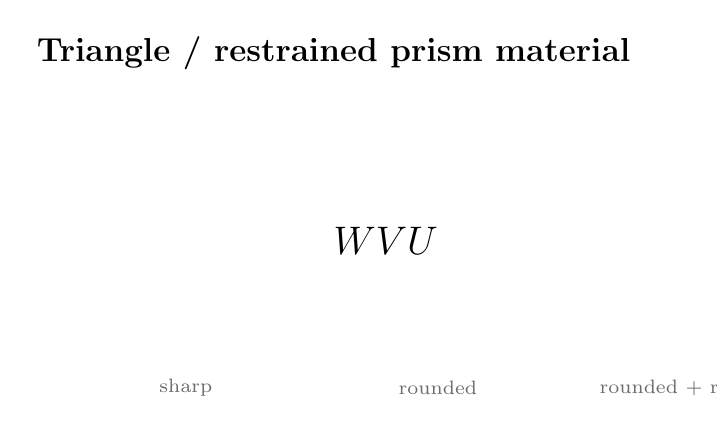
\begin{tikzpicture}[font=\sffamily]
  \node[font=\bfseries\large] at (0,2.55) {Triangle / restrained prism material};
  \tnvShape[shape=triangle,color=black!48,width=25mm,height=18mm,corner radius=0mm,font=\Large]{tri-sharp}{(-3.2,0)}{$W$}
  \tnvShape[shape=triangle,color=cyan!48!blue,width=25mm,height=18mm,corner radius=1.2mm,font=\Large,text color=white!92!black]{tri-soft}{(0,0)}{$V$}
  \tnvShape[shape=triangle,color=violet!64!black,width=25mm,height=18mm,corner radius=2.4mm,rotation=-90,font=\Large,text color=white!92!black]{tri-rotated}{(3.2,0)}{$U$}
  \node[font=\scriptsize,text=black!58] at (-3.2,-1.7) {sharp};
  \node[font=\scriptsize,text=black!58] at (0,-1.7) {rounded};
  \node[font=\scriptsize,text=black!58] at (3.2,-1.7) {rounded + rotated};
\end{tikzpicture}

% 4. Diamond: useful as a visually distinct, compact special tensor.
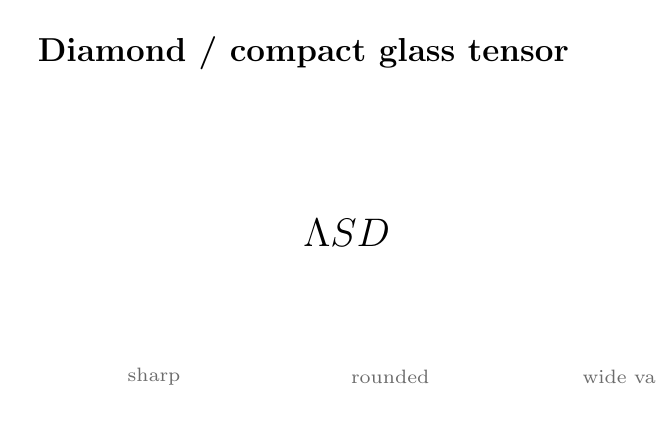
\begin{tikzpicture}[font=\sffamily]
  \node[font=\bfseries\large] at (0,2.45) {Diamond / compact glass tensor};
  \tnvShape[shape=diamond,color=black!48,width=22mm,height=17mm,corner radius=0mm,font=\Large]{dia-sharp}{(-3.0,0)}{$\Lambda$}
  \tnvShape[shape=diamond,color=violet!64!black,width=22mm,height=17mm,corner radius=1.1mm,font=\Large,text color=white!92!black]{dia-soft}{(0,0)}{$S$}
  \tnvShape[shape=diamond,color=blue!64!black,width=26mm,height=14mm,corner radius=2.0mm,font=\Large,text color=white!92!black]{dia-wide}{(3.2,0)}{$D$}
  \node[font=\scriptsize,text=black!58] at (-3.0,-1.65) {sharp};
  \node[font=\scriptsize,text=black!58] at (0,-1.65) {rounded};
  \node[font=\scriptsize,text=black!58] at (3.2,-1.65) {wide variant};
\end{tikzpicture}

\end{document}
